\documentclass[a4paper]{article}



    \usepackage[colorinlistoftodos]{todonotes}
 
	\usepackage[utf8]{inputenc}
	\usepackage[T1]{fontenc}
    \usepackage[frenchb]{babel}
    \usepackage{textcomp} 
	\usepackage[top=3cm,left=3cm,right=3cm,bottom=2cm]{geometry}
    \usepackage{lmodern}
    \usepackage{sectsty}
    \usepackage{nicefrac}
	\usepackage{graphicx}
    \usepackage{lastpage}
    \usepackage{fancyhdr}
    \usepackage{amsmath}
    \usepackage{amssymb}
    \usepackage{amsfonts}
    \usepackage{capt-of}
    \usepackage{caption}
    \usepackage{tikz}
    \usepackage{multirow}
    \usepackage{todonotes}
    \usepackage{verbatim}
    
    \usepackage{fancyvrb} % pour forcer les verbatim sur une seule page
    \usepackage{url}
    
    \newcommand\matlab{MATLab\textsuperscript{\textregistered}}




\title{Compte rendu de TP: Modélisation auto-régressive }

\author{Thomas Lechat \& Dinsenmeyer Alice}

\begin{document}
\maketitle



\section{Introduction}
Le but du TP est de mettre en application la théorie de la modélisation auto-régressive de systèmes vue pendant les cours de traitement du signal. Pour cela, un signal de bruit de structure est à disposition pour être analysé. Dans un premier temps, une modélisation du signal avec un modèle auto-régressif (AR) est effectuée. Le signal ainsi créé est comparé au signal source. Enfin une optimisation de la modélisation est réalisée au moyen du Critère d'Information d'Akaike ou de l'Erreur de Prédiction Linéaire.
Le code produit lors du TP est disponible en annexe A.


\section{Modélisation AR d'un signal de bruit de structure}
On appelle $b(t)$ la réponse impulsionnelle de la structure à modéliser. On cherche à estimer les paramètres d'un filtre permettant de modéliser le comportement vibratoire de la structure sur laquelle est mesurée le signal $b(t)$. Pour cela on utilise un modèle auto-régressif, le filtre recherché ne comporte que des pôles afin de modéliser les résonances de la structure. L'information du signal $b(t)$ peut être entièrement extraite de l'auto-corrélation du signal. On notera dans la suite cette auto-corrélation $R_{bb}(\tau)$. 
\bigskip
Une fois le système modélisé par un filtre avec des paramètres connus, on peut calculer la réponse en fréquence du filtre et la comparer à la réponse en fréquence de la structure. Si une différence est observée, il suffit alors de changer les paramètres du filtre pour retrouver la bonne réponse en fréquence: le changement de ces paramètres décrit le passage du système réel d'un état à un autre. Ce principe est représenté sur le schéma figure ~\ref{schema1}.

\begin{figure}[!h]
	\centering
	\includegraphics[scale=0.7]{schema_explicatif.png}
    \label{schema1}
    \caption{Schéma explicatif du principe de contrôle d'un système par modélisation auto-régressive.}
\end{figure}


\subsection{Calcul de l'auto-corrélation du signal réel}
On calcul tout d'abord l'auto-corrélation du signal $b(t)$. Pour cela, la fonction $xcorr$ de matlab est utilisée. Cette auto-corrélation contient toute l'information sur le signal $b$, elle est donc suffisante pour créer un filtre permettant de reproduire ce signal.

\subsection{Construction du filtre par algorithme du Durbin-Levinson}
La relation entre l'auto-corrélation de la réponse impulsionnelle du système réel et les paramètres du modèle est donnée par les équations de Yule Walker. Plusieurs algorithmes permettent ce calcul, l'algorithme de Durbin-Levinson a été utilisé dans le cadre du TP. La fonction matlab $levinson$ permet de calculer les coefficients du filtre ainsi que la variance idéale du bruit blanc à appliquer en entrée pour obtenir une réponse impulsionnelle se rapprochant au maximum de celle de la structure. Il suffit alors de calculer la réponse en fréquence du filtre pour pouvoir comparer modèle et système réel.

\bigskip
Un ordre du modèle doit être spécifié: celui-ci correspond au nombre de point pris de l'auto-corrélation de la réponse impulsionnelle pour calculer les coefficients du filtre. Cette ordre correspond donc aussi au nombre de paramètres du filtre. Dans la section suivante, on considère un modèle d'ordre $N=10$.

\section{Comparaison du modèle et du signal réel}
Une fois les coefficients du filtre déterminés, on a un modèle paramétrique permettant de caractériser le système réel. Il suffit alors de recalculer les coefficients si la réponse impulsionnelle du système réel change afin d'obtenir un jeu de paramètres décrivant le système au cours du temps.

On calcul donc la réponse impulsionnelle du filtre en lui appliquant un bruit blanc dont la variance est donné par l'algorithme de Durbin-Levinson. A partir de cette réponse impulsionnelle théorique, différentes quantités peuvent être comparéss.

\subsection{Comparaison des auto-corrélation}
L'auto-corrélation de la réponse impulsionnelle du filtre est tout d'abord calculée. Celle-ci est comparée à celle du système réel sur la figure ~\ref{autocorr}.

\begin{figure}[!h]
	\centering
	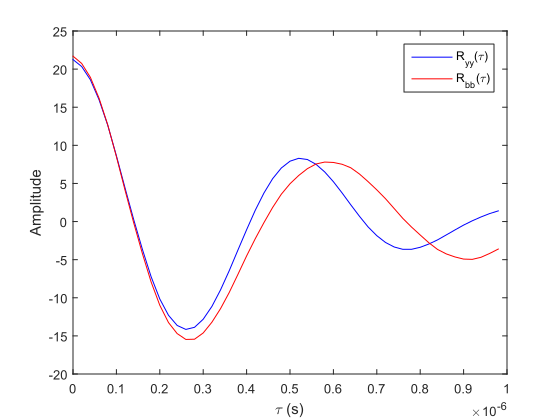
\includegraphics[scale=0.7]{autocorr.png}
    \label{autocorr}
    \caption{Comparaison des signaux réel et simulé par leur fonction d'auto-corrélation}
\end{figure}

Les auto-corrélations correspondent bien sur les premiers point puis divergent. Cela est dû au fait que c'est l'ordre du modèle qui fixe la longueur du signal devant être identique au 2 auto-corrélations.

\subsection{Comparaison des réponses en fréquence}
On compare maintenant les contenus en fréquentiels des réponses impulsionnelles du système réel et du filtre. Pour cela, les périodogrammes de Welch des 2 réponses impulsionnelles sont représentés figure ~\ref{dsp}. On ajoute aussi la densité spectrale de puissance théorique calculée pour le filtre.

\begin{figure}[!h]
	\centering
	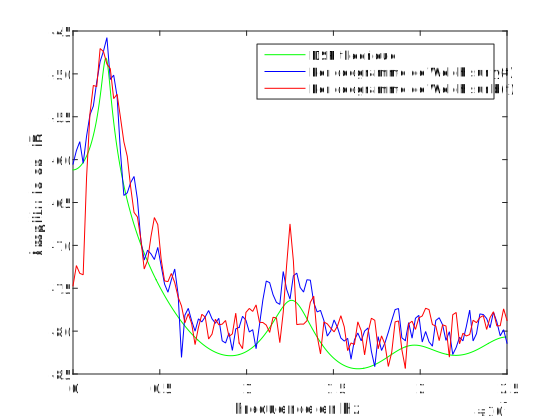
\includegraphics[scale=0.7]{dsp1.png}
    \label{dsp}
    \caption{Comparaison des signaux réels (en rouge) et simulés (en bleu et vert) par leurs contenu fréquentiel}
\end{figure}
Les périodogrammes sont calculés avec une fenêtre de Hanning de 256 points et un recouvrement de 50%.
Les 2 signaux semble bien avoir le même contenu fréquentiel. Par conséquent, le filtre est une bonne approximation du filtrage fait par le système réel.
On peut cependant remarquer que la deuxième résonance n'est pas très bien définie sur le filtre. Ce dernier point peut être corrigé en jouant sur l'ordre du filtre.

\subsection{Comparaison des signaux temporelles}
L'aspect des réponses impulsionnelles sont maintenant comparés sur la figure ~\ref{comp_temps}.

\begin{figure}[!h]
	\centering
	\includegraphics[scale=0.5]{comp_temps.png}
    \label{comp_temps}
    \caption{Comparaison des réponses impulsionnelles des signaux réel et simulé }
\end{figure}

Bien que jusqu'alors tout semble correspondre, les 2 signaux ne semble pas identiques dans le domaine temporel. On peut en déduire que le fait que 2 signaux disposent des mêmes caractéristiques statistiques n'entraîne pas nécessairement leurs ressemblance dans le domaine temporel. Cependant le filtre et le système réel ont bien tout deux les mêmes propriétés. 

\section{Optimisation du modèle par minimisation d'un critère test}
Le seul paramètre modifiable dans la modélisation est l'ordre du modèle. La section suivante a pour but de déterminer si un ordre optimal peut être trouvé pour notre problème. Pour cela, un critère doit être défini puis être minimisé. Dans la suite, on s'intéresse à 2 critères différents.


\subsection{critère d'Information d'Akaike}
Le premier critère est le critère d'Information d'Akaike. Celui-ci est donné par la formule suivante, ou $N$ est l'ordre du modèle:
\begin{equation}
AIC(N) = ln(\sigma ^2) = 2 N/M
\end{equation}

$M$ est le nombre de points du signal et $\sigma ^2$ la variance (calculée pour l'algorithme de Levinson) du bruit blanc mis en entrée du modèle auto-régressif. Il est à noter que ces critères (celui-ci comme le suivant) nécessitent de recalculer les coefficients du filtre ainsi que la variance en entrée. Cela est donc assez gourmand en temps de calcul et n'est pas nécessairement adapté à un contrôle en temps réel d'un système dynamique.
On trace le critère d'Information d'Akaike sur la figure ~\ref{criteres}.

\subsection{erreur de prédiction finale}
Le second critère s'exprime sous la forme suivante:
\begin{equation}
FPE(N) = \sigma ^2 \frac{M+N+1}{M-N-1}
\end{equation}

Celui-ci est aussi tracé figure ~\ref{criteres}.


\begin{figure}[!h]
	\centering
	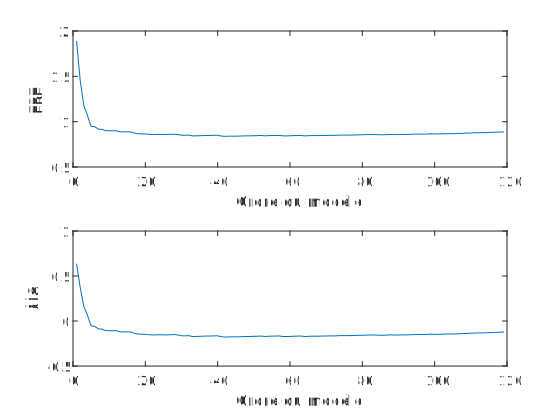
\includegraphics[scale=0.7]{criteres.png}
    \label{criteres}
    \caption{Critères d'erreur de prédiction finale et critère d'Information d'Akaike en fonction de l'ordre du modèle}
\end{figure}

Les 2 courbes possèdent un minimum, un ordre du modèle optimale peut donc bien être obtenu. Cependant, un modèle avec un faible nombre de paramètres est moins coûteux en temps de calcul, un compromis dois donc être trouvé entre justesse et rapidité. Ici le minimum des 2 critères se trouvent à un ordre du modèle environ égale a $N_{opti}=40$. Cependant dès $N=20$ l'erreur commise quand on augmente l'ordre ne semble plus significative. Il n'est donc pas nécessairement pertinent d'aller au delà et ce même si le minimum des critères n'est pas atteint.


\subsection{Comparaison de la densité spectrale de puissance optimisée et non-optimisée}
Une fois l'ordre du modèle optimal trouvé, il ne reste qu'a calculer les coefficients du filtre pour cette ordre pour finalement obtenir le périodogrammes de Welch théorique optimisé pour ce problème.

\begin{figure}[!h]
	\centering
	\includegraphics[scale=0.5]{otpi.png}
    \label{opti}
    \caption{Comparaison des signaux réel et simulé par leur contenu fréquentiel, avec optimisation de l'ordre du modèle.}
\end{figure}

Dans se cas de figure, la deuxième résonance est bien mieux définie que pour un modèle d'ordre $N=10$. L'ordre $N_{opti} = 42$ permet bien une meilleur estimation de la réponse en fréquence de la structure. Le modèle est cependant plus long en temps de calcul car il prend en compte un plus grand nombre de paramètres.

\section{Conclusion}
En conclusion, ce TP aura permis de mieux saisir les concepts vu en cours de traitement du signal au sujet des modèle auto-régressifs. L'utilisation de ce type de modèle à l'avantage de donner des paramètres que l'on peut analyser pour déterminer l'état d'un système physique alors qu'il serait trop compliqué (voir impossible) d'obtenir ces paramètres en utilisant une approche de physique mécanique. Il est cependant important de noter que les paramètres ainsi obtenus n'ont aucune réalité physique dans le sens ou ils découlent d'une modélisation mathématique et non pas d'une approche physique du système.

De nombreuses applications résultent de cette approche comme la prédiction linéaire ou encore le contrôle actif de certains systèmes.

 

\newpage
\section*{Annexe A}
\begin{verbatim}
%TP : modélisation autorégressive
%18/11/15

clear all; close all; clc

N=10; %ordre du filtre
load('bruit_structure.mat');   %chargement des données du système réel
L=length(b);

autocorr_b = xcorr(b,'biased');    %calcul de l'auto-corrélation 

%modele AR avec "Levinson-Durbin recursion"
%==========================================================================
[a_levinson, var_x]=levinson(autocorr_b(L:L+N-1),N);

%signal filtré x avec la fonction filter et les coeff précédemment trouvés
%===========================================================================
x=sqrt(var_x)*randn(1,L); %signal à l'entrée du filtre
y_levinson= filter(1,a_levinson,x); %signal à la sortie du filtre
autocorr_levinson=xcorr(y_levinson,'biased');

%comparaison des signaux par leurs autocorrélation
%==========================================================================
figure
plot(temps(1:5*N),autocorr_levinson(L:L+(5*N-1)),'b');
hold on
plot(temps(1:5*N), autocorr_b(L:L+(5*N-1)),'r');
legend('R_{yy}(\tau)','R_{bb}(\tau)')
%title('Comparaison des fonction d autocorrélation')
xlabel('\tau (s)');
ylabel('Amplitude');

%comparaison des signaux par leur contenu fréquentiel
%===========================================================================
Te=1/fe;
f=0:fe/L:fe/2-1; %axe fréquentiel

H_estime=0;
for n=1:N
H_estime= H_estime + a_levinson(n).*exp(-j*2*pi*n*Te*f); %fonction de transfert du filtre
end
H_estime=1./H_estime;
S_estime= (abs(H_estime)).^2.*var_x.*Te; %DSP théorique

K=256;
[ S_estime_welch, f_welch]=pwelch(y_levinson,hanning(K),K/2,K,fe); 
[ S_reel_welch, f_welch ]= pwelch(b,hanning(K),K/2,K,fe);

figure
plot(f,10*log10(S_estime),'g')
hold on
plot(f_welch,10*log10(S_estime_welch),'b')
hold on
plot(f_welch,10*log10(S_reel_welch),'r')
ylabel('Amplitude en dB')
xlabel('Fréquence en Hz')
legend('DSP theorique','Periodogramme de Welch sur y(t)','Periodogramme de Welch sur b(t)')
%title('Comparaison par le contenu fréquentiel')


%recherche de l'ordre du modele le plus pertinent
%==========================================================================
for i=2:120
    [a_levinson, var_x]=levinson(autocorr_b(L:L+i-1),i);
    FPE(i)= var_x* (L+i+1)/(L-i-1);
    AIC(i) = log(var_x)+2*i/L;
end

figure
subplot(2,1,1)
plot(FPE(2:end))
ylabel('FPE')
xlabel('Ordre du modèle')
subplot(2,1,2)
plot(AIC(2:end))
ylabel('AIC')
xlabel('Ordre du modèle')

[a min_FPE] = min(FPE(2:end));   % calcul des minimums des criteres
[a min_AIC] = min(AIC(2:end));


%recalcul de la DSP avec le bon nombre de coefficients
%==========================================================================
N=min(min_FPE,min_AIC);
[a_levinson, var_x]=levinson(autocorr_b(L:L+N),N);

H_estime=0;
for n=1:N
H_estime= H_estime + a_levinson(n).*exp(-j*2*pi*n*Te*f); %fonction de transfert du filtre
end
H_estime=1./H_estime;
S_estime= (abs(H_estime)).^2.*var_x.*Te;

figure
plot(f,10*log10(S_estime))
hold on
plot(f_welch,10*log10(S_reel_welch),'r')
title(['Comparaison des DSP avec N=' num2str(N)])
xlabel('Amplitude en dB')
ylabel('Fréquence de Hz')
legend('DSP theorique','Periodogramme de Welch sur b(t)')

\end{verbatim}

\end{document}